\let\negmedspace\undefined
\let\negthickspace\undefined
\documentclass[journal]{IEEEtran}
\usepackage[a5paper, margin=10mm, onecolumn]{geometry}
%\usepackage{lmodern} % Ensure lmodern is loaded for pdflatex
\usepackage{tfrupee} % Include tfrupee package

\setlength{\headheight}{1cm} % Set the height of the header box
\setlength{\headsep}{0mm}     % Set the distance between the header box and the top of the text

\usepackage{gvv-book}
\usepackage{gvv}
\usepackage{cite}
\usepackage{amsmath,amssymb,amsfonts,amsthm}
\usepackage{algorithmic}
\usepackage{graphicx}
\usepackage{textcomp}
\usepackage{xcolor}
\usepackage{txfonts}
\usepackage{listings}
\usepackage{enumitem}
\usepackage{mathtools}
\usepackage{gensymb}
\usepackage{comment}
\usepackage[breaklinks=true]{hyperref}
\usepackage{tkz-euclide} 
\usepackage{listings}
\usepackage{gvv}                                        
\def\inputGnumericTable{}                                 
\usepackage[latin1]{inputenc}                                
\usepackage{color}                                            
\usepackage{array}                                            
\usepackage{longtable}                                       
\usepackage{calc}                                             
\usepackage{multirow}                                         
\usepackage{hhline}                                           
\usepackage{ifthen}                                           
\usepackage{lscape}
\begin{document}

\bibliographystyle{IEEEtran}
\vspace{3cm}

\title{1.2.22}
\author{AI24BTECH11024-Pappuri Prahladha}
% \bigskip
{\let\newpage\relax\maketitle}

\renewcommand{\thefigure}{\theenumi}
\renewcommand{\thetable}{\theenumi}
\setlength{\intextsep}{10pt} % Space between text and floats


\numberwithin{equation}{enumi}
\numberwithin{figure}{enumi}
\renewcommand{\thetable}{\theenumi}


\textbf{Question}:\\
Rain is falling vertically at a speed of $35ms^{-1}$.Winds start blowing after sometime with a speed of $12ms^{-1}$ in east to west direction.In which direction should a boy waiting at a bus stop hold his umbrella ?
\\
\textbf{Solution: }
\begin{table}[h!]
    \renewcommand{\thetable}{1}
    \centering
    \begin{tabular}[12ptx]{ |c| c|}
\hline\textbf{Term} & \textbf{Description}\\
\hline
$\hat{i}$ and $-\hat{i}$ & Unit vectors along East and West directions \\

\hline
$\hat{j}$ and -$\hat{j}$ & Unit vectors along North and south directions\\
\hline
$\vec{V_{1}}$ or Vector 1 and $\vec{V_{2}}$ or Vector 2 & velocity vectors of Rain and Wind\\
\hline
$\vec{V_{3}}$ or Vector 3 & Resultant velocity vector of Rain and Wind\\
\hline
$\theta$ & Required angle with the horizontal\\
\hline
\end{tabular}
    \caption{Terms used}
    \label{TABLE 1:}
\end{table}


Velocity vector of rain:\\
\begin{equation}
\vec{V_{1}}=\begin{pmatrix}
0\\
-35
\end{pmatrix}
\end{equation}\\
Velocity vector of Wind:\\
\begin{equation}
\vec{V_{2}}=\begin{pmatrix}
-12\\
0
\end{pmatrix}
\end{equation}\\
The trajectory of Rain Drops is along the resultant velocity vectors of Rain and Wind.\\






The resultant velocity vector:\\
\begin{equation}
\vec{V_{1}}+\vec{V_{2}}=\begin{pmatrix}
    0\\
    -35
\end{pmatrix}
+
\begin{pmatrix}
    -12\\
    0
\end{pmatrix}\\
\end{equation}
\begin{equation}
    \vec{V_{3}}=\begin{pmatrix}
        -12\\
        -35
    \end{pmatrix}
\end{equation}
Let the origin be O:
\begin{equation}
    O=\begin{pmatrix}
        0\\
        0
    \end{pmatrix}
\end{equation}\\


The direction vector of AB is defined as:
\begin{equation}
    \vec{M}=\vec{B}-\vec{A}=k\begin{pmatrix}
        1\\
        m
    \end{pmatrix}
    \tag{1.1.1.1}
\end{equation}
Where m is the slope of AB.we can also say that\\

\begin{equation}
    \vec{m}\equiv k\begin{pmatrix}
        1\\
        m
    \end{pmatrix}
    \tag{1.1.1.2}
\end{equation}
So the direction vector of O and $v_{3}$ is:
\begin{equation}
    \vec{D}=\vec{V_{3}}-\vec{O}=\begin{pmatrix}
        -12\\
        -35
    \end{pmatrix}
=-12\begin{pmatrix}
    1\\
    \frac{35}{12}
\end{pmatrix}
\end{equation}\\
From equation 0.9 slope of direction vector $OV_{3}$ is\\
\begin{equation}
    Slope=\frac{35}{12}
\end{equation}
The required angle($\theta$) made by umbrella axis with the horizontal is;\\
\begin{equation}
    \theta=\tan^{-1}\brak{\frac{35}{12}}=71.075^\circ
\end{equation}\\

 $\therefore$ The boy hold the umbrella at an angle $71.075^\circ$ with           horizontal direction \\

 \begin{figure}[h!]
   \centering
   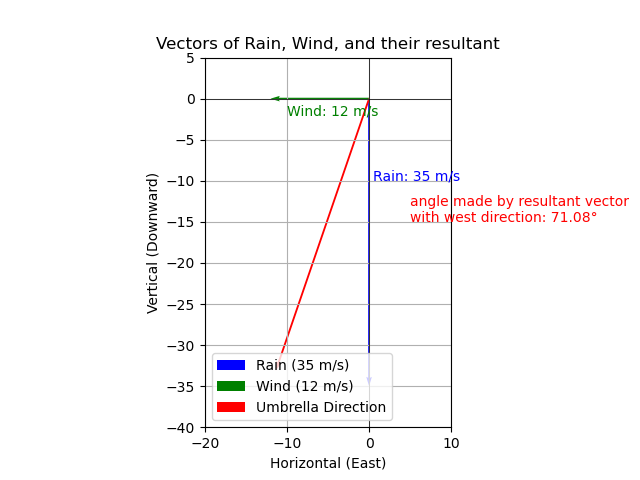
\includegraphics[width=0.7\linewidth]{figs/figure1.png.jpg}
   \caption{Plot showing the velocity vectors}
   \label{stemplot}
\end{figure}






\end{document}
